\begin{flushright}
    \textit{Лекция 13 (от 19.10)}
\end{flushright}
\pr
Из леммы $5$ очевидно следует необходимость (возьмем $a = b$).
\\
Докажем достаточность. Пусть $a \in G$, $z \in G$, $\gamma_{az}\in G$, $g(a) \in
\left\{ \sqrt[n]{f(z)} \right\}$. Тогда выполняется
\begin{equation}\label{(16.16)}
    g(z) = g(a) \sqrt[n]{\left| \frac{f(b)}{f(a)} \right|}\exp \left( \frac{i}{n} \Delta_{\gamma_{az}}\arg f(z) \right)
\end{equation}
Докажем регулярность такой ветви.
\\
Для замкнутых кривых экспонента примет значение $1$, а значит, $g(z)$ зависит
только от точки $z$. Очевидно, $\forall z \in G \ g(z)\in \left\{ \sqrt[n]{f(z)}
\right\}$. Докажем ее регулярность.
\\
Фиксируем произвольную $z_1 \in G$; тогда $\exists B_\varepsilon(z_1) \subseteq G$
такой, что
\begin{equation}\label{(16.17)}
    \forall z \in B_\varepsilon(z_1) \ g(z) = g(z_1) \sqrt[n]{\left| \frac{f(z)}{f(z_1)} \right|}\exp \left( \frac{i}{n} \Delta_{\gamma_{z_1z}}\argt f(z) \right)
\end{equation}
$B_{\varepsilon}(z_1)$ односвязна, значит, по лемме $2$
$\Delta_{\os{\circ}{\gamma}}\argt f(z) = 0$ для любой замкнутой
$\os{\circ}{\gamma} \subseteq B_\varepsilon(z_1)$. Но
\begin{align*}
  & g(z) = \exp \left( \frac{i}{n} h(z) \right)
\end{align*}
\begin{align*}
  & h(z) = \ln \left| f(z) \right| + i \left(\psi_0 + \Delta_{\gamma_{z_1z}}\argt f(z)\right), \ \psi_0 \in \Arg f(z_1)
\end{align*}
\begin{equation}\label{(16.18)}
    g(z_1) = \sqrt[n]{\abs{f(z_1)}} \exp\left( \frac{i}{n}\psi_0 \right)
\end{equation}
В $B_\varepsilon(z_1)$ есть регулярная ветвь $\Ln f(z)$, причем $h(z)$~--- та
самая ветвь, значит, $g(z)$ регулярна в $B_\varepsilon(z_1)$.
\\
В силу произвольности выбора $z_1$ показали регулярность во всей $G$.
\corollary
Если $h(z)$, $g(z)$~--- регулярные ветви $\Ln f(z)$ и $\left\{ \sqrt[n]{f(z)}
\right\}$ соответственно в $G$, то
\begin{equation}\label{(16.19)}
    h'(z) = \frac{f'(z)}{f(z)}
\end{equation}
\begin{equation}\label{(16.20)}
    g'(z) = \frac{f'(z)}{n\left( g(z) \right)^{n-1}}
\end{equation}
\pr
\begin{align*}
  & e^{h(z)} \equiv f(z) \rightarrow h'(z)e^{h(z)} \equiv f'(z) \Rightarrow h'(z) \equiv \frac{f'(z)}{f(z)}
\end{align*}
\begin{align*}
  & (g(z))^n \equiv f(z) \Rightarrow n(g(z))^{n-1}g'(z) \equiv f'(z) \Rightarrow g'(z) = \frac{f'(z)}{n\left( g(z) \right)^{n-1}}
\end{align*}
\section{$\S 17.$ Примеры вычисления регулярных ветвей.}
\Example
\begin{align*}
  & \left\{ \sqrt[4]{z^3(z+1)} \right\}, \ G = \CC \setminus[-1;0]
\end{align*}
Если ветвь существует, то
\begin{align*}
  & g_1(2) = i \sqrt[4]{24}
\end{align*}
При этих условиях найти $g_1(i)$, $g'_1(i)$.
\nonum
Заметим: $f(z) = z^3(z+1)$, $n=4$. Видим, что в $G$ $f(z) \neq 0$.
\\
$\forall \os{\circ}{\gamma} \subseteq G$~--- замкнутой~--- рассмотрим
$\Delta_{\os{\circ}{\gamma}}\argt f(z)$.
\begin{align*}
  & \Delta_{\os{\circ}{\gamma}}\argt f(z) = \Delta_{\os{\circ}{\gamma}}\argt z^3(z+1) = 3 \Delta_{\os{\circ}{\gamma}}\argt z + \Delta_{\os{\circ}{\gamma}}\argt (z-1)
\end{align*}
\begin{figure}[h!]
		\centering
		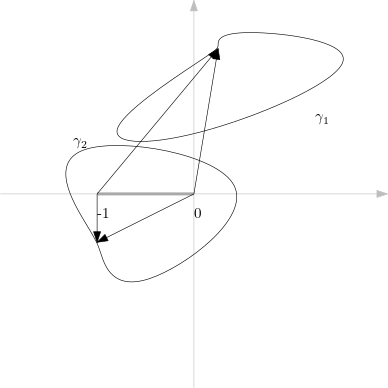
\includegraphics[scale=0.5]{Ex1.png}
		\label{fig:17.1}
\end{figure}
На кривых вида $\gamma_1$ (не опоясывающих разрез) приращение обоих аргументов
равно нулю (а значит, и суммарное), а на кривых вида $\gamma_2$ приращение
аргумента составит $8 \pi$. Оба случая удовлетворяют условию существования
регулярных ветвей.
\\
Докажем строго. Пусть $\os{\circ}{\gamma} = z(t)$, $t \in [0;1]$, $z(0) = z(1) =
z_0 \in \gamma$, $z(t, \alpha) = z(t) - \alpha$, $\alpha \in [-1;0]$. $\forall
(t, \alpha) \ z(t, \alpha) \neq 0$, $\forall \alpha \ z(1, \alpha) = z(0,
\alpha) = z_0 - \alpha$. Значит, по теореме $3$ $\S 14$ $I(\alpha) =
\Delta_{[0;1]}\argt z(t, \alpha) = const$, т.~е.
\begin{align*}
  & \Delta_{[0;1]} \argt z(t) = \Delta_{[0;1]} \argt(z(t) + 1) = \Delta_{\os{\circ}{\gamma}}z = \Delta_{\os{\circ}{\gamma}}(z+1) = 2 \pi k(\os{\circ}{\gamma})
\end{align*}
\begin{align*}
  & \Delta_{\ogamma} \argt f(z) = 4 \Delta_{\ogamma} \argt z = 8 \pi
\end{align*}
Желаемое условие выполняется.
\\
Значит,
\begin{align*}
  & g_1(z) = g_1(2) \sqrt[4]{\frac{\left| z^3(z+1) \right|}{24}} \exp \left( \frac{i}{4}\left( \Delta_{\gamma{2z}}\argt f(z) \right) \right)
\end{align*}
\begin{align*}
  & g_1(i) = g_1(2) \sqrt[4]{\frac{\left| i^3(i+1) \right|}{24}} \exp \left( \frac{i}{4}\left( \Delta_{\gamma_{2,i}}\argt f(z) \right) \right) = 2^{\frac{1}{8}}i\exp \left( \frac{i}{4} \left( 3\Delta_{\gamma_{2,i}}\argt z + \Delta_{\gamma_{2,i}} \argt (z+1) \right) \right) = \\
  & = 2^{\frac{1}{8}}i\exp \left( \frac{i}{4} \left( 3\frac{\pi}{2} + \frac{\pi}{4} \right) \right) = 2^{\frac{1}{8}}i\exp \left( \frac{7i\pi}{16} \right) =  2^{\frac{1}{8}}e^{\frac{15i\pi}{16}}
\end{align*}
\begin{align*}
  & g_1'(z) = \frac{4z^3+3z^2}{4g_1^3(z)}
\end{align*}
\begin{align*}
  & g_1'(i) = \frac{-4i -3}{4\cdot 2^{\frac{3}{8}}e^{\frac{45i\pi}{16}}} = -(4i+3)2^{-\frac{19}{8}}e^{-\frac{13i\pi}{16}}
\end{align*}
\Example
\begin{align*}
  & \Ln (1-z^2), \ G = \CC \setminus (-\infty; 1]
\end{align*}
Если ветвь существует, то
\begin{align*}
  & \Img h\left( \frac{i}{5} \right) = 0
\end{align*}
При этих условиях найти разложение $h$ в ряд Тейлора по степеням $(z+i)$,
область, где $h(z) = S(z)$~--- сумма своего ряда Тейлора, его радиус сходимости
$R$ и $S\left( \dst \frac{i}{5} \right)$.
\nonum
$G$ односвязна. Заметим: $f(z) = 1-z^2 \neq 0$ в $G$.
\\
$\forall \gamma \subseteq G$ рассмотрим $\Delta_{\gamma}\argt f(z)$.
\begin{align*}
  & h(z) = \ln \left| z \right| + i \Img h(z)
\end{align*}
\begin{align*}
  & h\left( \frac{i}{5} \right) = \ln \frac{26}{25}
\end{align*}
\begin{figure}[h!]
		\centering
		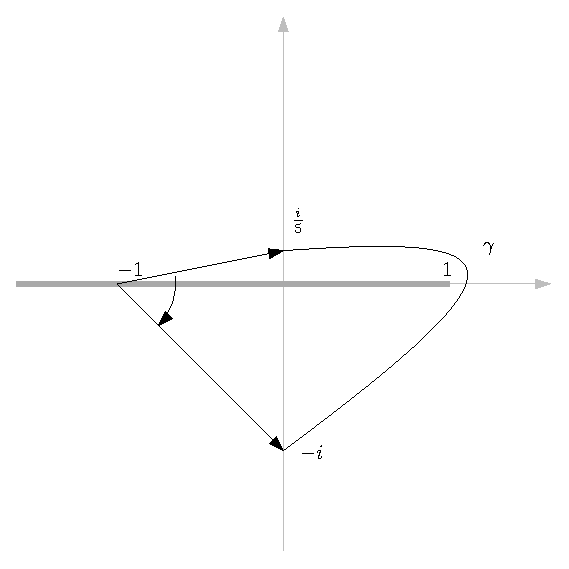
\includegraphics[scale=0.75]{Ex1.eps}
		\label{fig:17.2}
\end{figure}
\begin{align*}
  & h(-i) = \ln \frac{26}{25} + \ln \left| \frac{2}{\frac{26}{25}} \right|+ i\left( \Delta_{\gamma_{\frac{i}{5}, -i}}\argt (z+1) + \Delta_{\gamma_{\frac{i}{5}, -i}}\argt (z-1) + \Delta_{\gamma_{\frac{i}{5}, -i}}\argt (-1) \right) = \ln 2 - 2 i \pi
\end{align*}
Положим $\zeta = z+i$, $h(z) = h(\zeta - i) = \tilde{h}(\zeta)$. Тогда
$\tilde{h}(0) = h(-i) = \ln 2 - 2 i \pi$. Хотим разложить это в ряд.
\begin{align*}
  & \tilde{h}(\zeta) \in \Ln (1-(\zeta - i)^2) = \Ln(2+2i\zeta - \zeta^2) = \Ln \left(2\left( 1 - \frac{\zeta}{1-i} \right)\left( 1 - \frac{\zeta}{1+i} \right) \right) = \Ln 2 + \\
  & \Ln \left( 1 - \frac{\zeta}{1-i} \right) + \Ln \left( 1 - \frac{\zeta}{1+i} \right)
\end{align*}
Из теоремы об обратной функции
\begin{align*}
  & h^*_k(z) \in \Ln (1+z), \ \left| z \right| < 1 \Rightarrow h^*_k(z) = 2 i \pi k + \sum_{n=1}^\infty \frac{(-1)^{n+1}}{n} z^n, \ \left| z \right| < 1
\end{align*}
Рассмотрим
\begin{align*}
  & h_+(\zeta) \in \Ln \left( 1 - \frac{\zeta}{1+i} \right), \ \left| \zeta \right| < \sqrt{2}, \ h_+(0) = 0 \Rightarrow h_+(\zeta) = - \sum_{n=1}^\infty \frac{\zeta^n}{n(1+i)^n}, \ \left| \zeta \right| < \sqrt{2}
\end{align*}
\begin{align*}
  & h_-(\zeta) \in \Ln \left( 1 - \frac{\zeta}{1-i} \right), \ \left| \zeta \right| < \sqrt{2}, \ h_-(0) = 0 \Rightarrow h_-(\zeta) = - \sum_{n=1}^\infty \frac{\zeta^n}{n(1-i)^n}, \ \left| \zeta \right| < \sqrt{2}
\end{align*}
Заметим, что $\sqrt{2}$~--- максимальный радиус, т.~к. выходим на особую точку.
Видим:
\begin{align*}
  & \tilde{h}(\zeta) - h_+(\zeta) - h_-(\zeta) = \ln 2 + 2 i \pi k(\zeta)
\end{align*}
В правой части функция непрерывная, в левой ступенчатая, значит, $k = const$.
Найдем ее:
\begin{align*}
  &  \tilde{h}(0) - h_+(0) - h_-(0) = \ln 2 + 2 i \pi k = \ln 2 - 2 i \pi
\end{align*}
Значит, $k = -1$.
\\
Значит,
\begin{align*}
  & \tilde{h}(\zeta) = - \sum_{n=1}^\infty \frac{\zeta^n}{n(1+i)^n} - \sum_{n=1}^\infty \frac{\zeta^n}{n(1-i)^n} + \ln 2 - 2 i \pi
\end{align*}
\begin{align*}
  & h(z) = - \sum_{n=1}^\infty \frac{1}{n}\left( \frac{1}{(1+i)^n}+ \frac{1}{(1-i)^n}\right)(z-i)^n + \ln 2 - 2 i \pi, \ \left| z-i \right|< \sqrt{2}
\end{align*}
Видим, что $S(z)$ регулярна на $\left| z-i \right|< \sqrt{2}$; $S(z)$ и $h(z)$
есть регулярные ветви логарифма. Но также можем заметить, что часть разреза
лежит внутри круга сходимости. Тогда
\begin{align*}
  & \forall x \in (-1;1) \ h(x + i0) = h(x-i0) + i\Delta_{x+i0, x-i0}\argt h(z) = h(x-i0) + 2 i \pi \neq h(x-i0)
\end{align*}
Значит, внутри круга при положительной мнимой части $h(z) = S(z) + 2 i \pi$, а
при отрицательной мнимой части $h(z) = S(z)$.
\\
Значит,
\begin{align*}
  & S\left( \frac{i}{5} \right) = \ln \frac{25}{26} - 2 i \pi
\end{align*}
\begin{align*}
  & S'\left( \frac{i}{5} \right) = \left. \frac{-2z}{(1-z^2)} \right|_{z=\frac{i}{5}} = \frac{-2i\cdot 25}{5\cdot 26} = -\frac{5i}{13}
\end{align*}
\Def
Пусть $a, b \in \CC$, $a \neq 0$. Тогда
\begin{equation}\label{(17.1)}
    \left\{ a^b \right\} = \exp\left( b \Ln a\right)
\end{equation}
\Exse
Если $b = n$ или $b = \dst \frac{1}{n}$, $n\in \NN$, то \eqref{(17.1)} описывает
$a^n$ или $\left\{ \sqrt[n]{a} \right\}$ соответственно.
\Example
Разложить в ряд Тейлора регулярные ветви функции
\begin{align*}
  & \left\{ (1+z)^b \right\}, \ \left| z \right|<1
\end{align*}
\nonum
По определению,
\begin{align*}
  & (1+z)^b = \exp \left( b \Ln (1+z) \right)
\end{align*}
В силу существования регулярных ветвей у логарифма в этом круге ($h_k(0) = 2 i
\pi k$, $h_k$~--- регулярные ветви), то есть и регулярные ветви данной функции
будут существовать и иметь вид $w_k(z) = \exp \left( b h_k(z) \right)$.
\Exse
Доказать, что любая регулярная ветвь этой функции имеет такой вид.
\\
Вычислим производные $w_k$.
\begin{align*}
  & w_k(0) = e^{2bi\pi k}
\end{align*}
\begin{align*}
  & w_k'(z) = w_k(z) \frac{b}{1+z} \Rightarrow w_k'(0) = be^{2bi\pi k}
\end{align*}
\begin{align*}
  & w_k''(z) = w_k(z) \frac{b(b-1)}{(1+z)^2} \Rightarrow w_k''(0) = b(b-1)e^{2bi\pi k}
\end{align*}
\begin{align*}
  & w_k^{(n)}(z) = w_k(z) \frac{b(b-1)\dots(b-n+1)}{(1+z)^n} \Rightarrow w_k^{(n)}(0) = b(b-1)\dots(b-n+1)e^{2bi\pi k}
\end{align*}
\begin{align*}
  & w_k(z) = w_k(0)\sum_{n=0}^\infty C_b^nz^n
\end{align*}
\Example
Разложить в ряд Тейлора функцию
\begin{align*}
  & g \in \left\{ \sqrt[3]{1-z^2} \right\}, \ B_1(0), \ g(0) = \exp \left( \frac{2 i \pi}{3} \right)
\end{align*}
\nonum
По аналогии с предыдущим примером,
\begin{align*}
  & g(z) = \exp \left( \frac{2 i \pi}{3}\sum_{n=1}^\infty C_{\frac{1}{3}}^n(-1)^n z^{2n} \right)
\end{align*}
\Example
Разложить в $\os{\circ}{B}_1(\infty)$ в ряд Лорана регулярные ветви функции
\begin{align*}
  & \sets{\sqrt[4]{z^3(z+1)}}
\end{align*}
\nonum
\begin{align*}
  & \os{\circ}{B}_1(\infty) = \left\{ z \mid \left| z \right| > 1\right\}\subseteq \CC \setminus [-1;1]
\end{align*}
По аналогии с примером $1$
\begin{align*}
  & g_k(z) = \sqrt[4]{24}\exp \left( \frac{i\pi k}{2} \right)
\end{align*}
При $x > 2$, $x \in \RR$
\begin{align*}
  & g_0(x) = \sqrt[4]{x^3(x+1)} = x \sqrt[4]{1+\frac{1}{x}} = x \sum_{n=1}^\infty C_{\frac{1}{4}}^n\left( \frac{1}{x} \right)^n = S(x)
\end{align*}
\begin{align*}
  & \forall x \in \RR \cap (2; \infty) \ g_0(x) = S(x)
\end{align*}
Обе функции $S(z)$ и $g_0(z)$ регулярны, и по теореме единственности $g_0(z) =
S(z)$, а значит, искомый ряд Лорана будет иметь вид
\begin{align*}
  & z \sum_{n=1}^\infty C_{\frac{1}{4}}^n\left( \frac{1}{z} \right)^n
\end{align*}
